% !Mode:: "TeX:UTF-8"
% !TEX program  = xelatex

%\documentclass{cumcmthesis}
\documentclass[withoutpreface,bwprint]{cumcmthesis} %去掉封面与编号页,电子版提交的时候使用。

\usepackage{zhlipsum}
\usepackage{gbt7714}
\usepackage{setspace}
\usepackage{chemfig}

\usepackage{graphicx} %use graph format
\usepackage{epstopdf}
\usepackage[framemethod=TikZ]{mdframed}
\usepackage{url}   % 网页链接
\usepackage{subcaption} % 子标题
\title{古代玻璃制品的成分分析与鉴别}
\tihao{C}
\baominghao{}
\schoolname{}
\membera{}
\memberb{}
\memberc{}
\supervisor{}
\yearinput{2022}
\monthinput{09}
\dayinput{18}

\begin{document}

\maketitle
\begin{abstract}

本文主要研究了古代两种类型玻璃的物理特征和化学成分,
提取与文物样品表面风化有关的风化化学成分,
以及对未知类别的玻璃进行鉴别,并且划分到亚类当中。

针对问题一,对附件中的表单一、二的数据进行合并和预处理后,
采用控制变量的方法,一一探寻文物样品表面风化与各个物理特征的关系,
通过设定\textbf{相对易风化程度系数$W$和$P$},
以及绘制图表,找到其中的统计规律,并查找文献分析该规律出现的原因,
本文充分考虑了玻璃烧制环境、助熔剂类别、埋藏环境等因素对文物风化的影响。
在探寻文物是否风化和其化学成分含量之间关系的统计规律时,
本文为了减小数据缺失等因素的影响,使用\textbf{独立样本$t$检验进行方差分析},
来判断在风化前后,含量有显著变化的化学成分,
并将这些化学成分定为风化化学成分,通过观测图表获得统计规律。
最后,在独立样本$t$检验所得的结果之上,
对风化点风化前的化学成分含量进行预测,
根据均值差$\Delta_i$构造模型,从而求解各个风化点未风化时的化学成分含量。

针对问题二,本文分别从化学特征和物理特征着手,
得出高钾玻璃与铅钡玻璃的分类规律,对于化学特征,
本文绘制了两种玻璃类型之间,各个化学成分对比的箱型图,
共14张,在筛选后得到了5张有强分类意义的箱型图,
\textbf{分别为\chemfig{SiO_2}, \chemfig{K_2O},\chemfig{PbO},\chemfig{BaO} ,\chemfig{SrO},}
并将其作为主要特征参与后续的训练。
其中\chemfig{PbO}可以将高钾玻璃和铅钡玻璃完全划分。
由于本问还要求选择合适的化学成分,对两种类型的玻璃进行亚类划分,
本文先使用Davies Bouldin Index确定簇类数量,其最佳解为$k=5$。
然后运用\textbf{$K$-menas聚类算法},将所有样本分成5个聚类。
最后将五种亚类输入到\textbf{CART决策树}中,让它基于不同的化学成分,
进行亚类的特征提取。该亚类分类模型的\textbf{AUC值达到98\%},接近完美分类器。

针对问题三,由于本问的玻璃样本无类别特征,
本文需要对附件表单三中的文物样本,
先进行\textbf{高钾玻璃和铅钡玻璃的类别划分},
然后使用问题二中训练的亚类分类模型,
对这些文物样本进行进一步的亚类划分。
我们通过给样本一定的\textbf{随机扰动}的方式探究决策树的敏感性和鲁棒性。

针对问题四,本文选取在问题二的箱型图选择中,
获得的五种化学成分,针对同种类型的玻璃,
两两化学成分组合绘制散点图。观测这些散点图,
选取残差较小、直线拟合较好、有明显关联关系的图,
进行化学成分关联关系特征提取。
最后,本文比较两种玻璃类型中的同种散点图趋势关系,得出其差异性。
\keywords{独立样本$t$检验\quad Davies Bouldin Index \quad $K$-means聚类算法 \quad CART决策树}
\end{abstract}


\section{问题重述}

\subsection{问题背景}
由于中国考古行业的不断发展,近几年来,
我国出土了数千件古代玻璃制品,
其出土地点主要沿丝绸之路分布。
在古代,玻璃器物的体积都较小,
具有极强的便携性,在往来贸易中,
由西方商人随身携带而传入中国。
我国古代人民在吸收其技术后,加以改进,
形成了与外来玻璃制品相似,
但化学成分不同的玻璃,
最具有代表性的是楚文化的铅钡玻璃,
以及流行于我国岭南等区域的高钾玻璃,
两种玻璃的差别主要在于添加的助熔剂不同。
古代玻璃在经过长时间的埋藏后,
会因为玻璃本身的化学组成和其外部保存环境而发生风化。
风化严重的玻璃表面会被风化物完全覆盖,
使其原貌几乎无法辨认,
并且化学成分也会发生改变。


\subsection{问题提出}
已知一批我国古代玻璃制品的相关数据,
其中包含这些文物的分类信息、外观、主要成分和风化情况
由于技术限制,部分成分不能被显式地检测到。
根据题意,我们将各个问题拆分为若干小问:

\noindent {\bfseries 问题1:}
\begin{enumerate}
    \item 对玻璃文物表面风化与其物理特征(包含玻璃类型、纹饰和颜色)进行分析。
    \item 结合其玻璃类型,分析化学成分含量与风化程度的统计规律。
    \item 根据风化点检测数据,预测其风化前的化学成分含量。
\end{enumerate}


\noindent {\bfseries 问题2:}
\begin{enumerate}
    \item 分析高钾玻璃和铅钡玻璃的分类规律。
    \item 对不同类别的玻璃,选择合适的化学成分,建立数学模型进行亚类划分,并给出具体划分方法和划分结果。
    \item 分析该分类结果的合理性和敏感性。
\end{enumerate}


\noindent {\bfseries 问题3:}
\begin{enumerate}
    \item 根据未知类别的玻璃文物的化学成分,预测其所属类型。
    \item 分类结果的敏感性进行分析。
\end{enumerate}

\noindent {\bfseries 问题4:}
\begin{enumerate}
    \item 针对同种玻璃,分析其化学成分之间的关联关系。
    \item 针对不同种玻璃,分析化学成分之间关联关系的差异性。
\end{enumerate}


% TODO
\section{问题分析}

\subsection{对问题一的分析}
1.
本问要求我们分别分析文物表面风化和玻璃类型的关系,
文物表面风化和纹饰的关系,
以及文物表面风化和颜色的关系。
针对该问题,
首先我们对玻璃类型和表面纹饰拟定了两个相对易风化程度系数,
据此来判断文物表面风化与否与它的关系,
并查找文献解释这其中的原因。
在分析颜色和文物表面风化之间的关系时,
我们不仅仅是考虑颜色和是否风化这两个变量,
我们在引入玻璃类型作为第三个变量的基础上,
通过统计数据、绘制图表得到了一个不同颜色对文物风化的影响,
并根据文献合理推断了其中原因。

2.
本问需要我们结合玻璃类型,
分析玻璃文物是否风化和样品表面的化学成分含量的关系,
并归纳出统计规律。
考虑到玻璃文物表面风化受诸多因素的影响,
并且附件中有些数据因检测手段等原因而缺失,
我们采用独立样本t检验来判断哪些化学成分在风化后变化显著,
将这些显著变化的化学成分定为风化化学成分,并得出其统计规律。

3.
本问期望我们预测各个风化点,
过去未风化时的化学成分含量。
在上一问中,我们已经获取了风化化学成分,
并用独立样本t检验证了这些化学成分的均值存在差异且有意义,
因此我们假设风化前后只有这些风化化学成分的含量发生改变,
根据同种玻璃风化前后某种风化化学成分的均值差$\Delta$,
我们构造了一个可以用于预测风化前化学成分含量的模型,
带入风化后的含量,最终我们得到了各个风化点的过去化学成分的含量。

\subsection{对问题二的分析}

1.
本问要求得出两种类型的玻璃的分类规律。
我们先对化学特征进行分析,
针对两种玻璃的各个化学成分绘制箱型图,
并加以比较。在14张图中,
我们筛选出了5个最具有分类意义的化学成分,
其中有一种化学成分可以将两种玻璃类型完美分类,
据此我们得出了不同种玻璃的分类规律。
此外,我们还发现在对不同种玻璃分类时,
纹饰的类型也具有一定的分类规律。

2
这一问要求我们对两种类型的玻璃进行亚类划分,
并给出具体的划分方法和划分结果。
对于该问题,我们采用$K$-means聚类算法来获得亚类,
在此之前我们使用Davies-Bouldin Index (DBI) 
来确定$K$-means中簇类的数量,通过不断地迭代计算,
我们获得了五个簇类,将此结果输入到决策树CURT中,
获得这五种亚类基于不同化学成分的划分方法及具体结果。

3.
这一问是分析上一问分类结果合理性和敏感性。
我们回顾整个模型的搭建过程,认为这之间各个环节是安排合理的、精密连结的,
因此上一问经过该模型得出的分类结果具有合理性。
通过绘制决策树的ROC-AUC曲线,我们得出它接近于一个完美分类器。


\subsection{对问题四的分析}

1.
本问需要在在问题二的基础上,
对未知类别的玻璃文物进行化学成分分析,
并将其划分到合适的亚类当中。
利用问题二中第二小问得到的决策树模型,
将附录三中的数据输入到其中,
即可得出这些未知类别的玻璃文物所属类型。

2.
对上一小问的分类进行敏感性分析。


\subsection{对问题三的分析}
  
1.该问是分析不同种玻璃文物样品之间,化学成分的关联关系。
  
2.本问针对上一问得到的不同类别之间的化学成分关联关系,分析其差异性。




\section{模型假设}

\begin{enumerate}
    \item 因此我们假设风化前后只有这些风化化学成分的含量发生改变
    \item 文物是否风化,可能受到多种化学成分的影响,但我们假设各化学成分之间没有交互作用,且我们的数据是连续的、呈正态分布的。
    \item 在独立样本$t$ 检验中,我们首先假设 同种玻璃的某种物质风化前后的均值相等
    \item 我们假设除了风化化学成分以外的其他化学成分所占百分比不会发生改变
\end{enumerate}


%\section{符号说明}

% 本文所使用的变量符号及其含义如表\ref{tab:sign}所示。

%\begin{table}[!htbp]
    %\caption{本文符号}\label{tab:sign} \centering
    %\begin{tabular}{p{1.5cm}p{5cm}|p{1.5cm}p{5cm}}
        %\toprule[1.5pt]
        %符号           & 含义                    & 符号              & 含义            \\
        %\midrule[1pt]
        %$x^{<i>}_{id}$ & 样本 $i$ 的文物唯一编号 & $x^{<i>}_{color}$ & 样本 $i$ 的颜色 \\
        %\bottomrule[1.5pt]
    %\end{tabular}
%\end{table}



\section{数据清洗及探索性数据分析}

\subsection{数据合并}

附件``表单一''中提供了``文物编号''一数据,
附件``表单二''中提供了``文物采样点''一数据,
其中``文物采样点''中包含了``文物编号''的特征,
我们从``文物采样点''中提取了``文物编号'' 作为文物的唯一识别编号,
并使用该特征将两张表连接,将文物的物理特征和化学特征整合。


\subsection{缺失值处理}
对于附件``表单一''提供的数据,
我们使用pandas \cite{reback2020pandas} 查找数据中的缺失值,
在特征``颜色''一列中,
发现4处缺失值,根据题意,
颜色对于玻璃风化程度的判定有着重要意义,
故采用\textbf{丢弃缺失值}的方式处理。
对于附件``表单二''提供的数据,
存在大量的缺失值,根据题意``空白处表示未检测到该成分'',
我们认为是该种元素的含量过低导致,
故使用将缺失值填充为$ 0 $ 的方式处理。


\subsection{异常值处理}
考虑到检测手段等原因可能导致其成分比例的累加和非 100\% 的情况,
根据题意,成分比例累加和介于 85\% \textasciitilde 105\%之间的数据视为有效数据,
经过筛选,共有两个样本的成分比例累加小于85\%,
视为无效数据,并将其丢弃。

\section{问题一的建模与求解}

\subsection{玻璃文物表面风化与其物理特征的关联性分析}
根据题目要求,
我们需要对玻璃文物的表面风化和它的玻璃类型、纹饰和颜色之间的关系进行分析,
我们将玻璃的类型、纹饰和颜色归纳为这些玻璃文物的物理特征。
我们依次观察数据和绘制图表,最终得到了文物表面风化和玻璃类型的关系,
文物表面风化和纹饰的关系,以及文物表面风化和颜色的关系。

\subsubsection{文物表面风化和玻璃类型的关系}

为了研究文物表面风化和玻璃类型的关系,
我们对附件一中的数据观测、分析,
得到了不同种类玻璃的相对易风化程度系数$W$
\begin{equation}
    W = \dfrac{C_w}{C_s}
\end{equation}
其中,$C_w$是该玻璃类型中的已风化玻璃数量,
$C_s$是该玻璃类型的所有样本总数。通过绘制柱状图(\ref{bb})我们发现,
铅钡玻璃相对于高钾玻璃更易风化。

通过查找文献,我们发现由于铅钡玻璃中含有大量的Pb元素,
它极易于与周围环境的氧气、\chemfig{CO_2}和\chemfig{H_2O}发生化学反应,
生成沉淀物\chemfig{PbCO_3 \cdot Pb{(}OH{)}_2} \cite{yijianzhanguoshiqibaleng}。

\begin{equation}
    \chemfig{4Pb + 2O_2 + 2CO_2 + 2H_2O = 2PbCO_3 \cdot Pb{(}OH{)}_2}
\end{equation}

而由草木灰作为助熔剂的高钾玻璃,
由于植物体本身含有一定量的稀土元素,
使高钾玻璃相对于铅钡玻璃而言更耐高温或耐腐蚀\cite{gudaibolicailiao}\cite{wedepohl2010chemical}。

\subsubsection{文物表面风化和纹饰的关系}
为了研究文物表面风化和不同纹饰的关系,
我们对具有不同纹饰的玻璃进行数据分析,
得到了不同纹饰的玻璃的相对易风化程度系数$P$:

\begin{equation}
    P = \dfrac{D_w}{D_s}
\end{equation}

其中,$D_w$是该纹饰中的已风化玻璃数量,
$D_s$是该纹饰中的所有样本总数。
在绘制直方图$\ref{bb}$后我们发现,
纹饰C比纹饰A更易风化,
而纹饰B的相对易风化程度为100\%。
由于纹饰B的相对易风化程度过高,
我们又单独观测了纹饰B的数据,
发现纹饰B只在高钾玻璃中出现,
并且这些玻璃全都易风化。

我们在网上查找了研究古代玻璃的论文资料和古代玻璃出土文物的图片,
我们认为纹饰B是玻璃珠形状的,大致成球形,中间穿孔\cite{yunnanluliangxianxueguanbao}。
对于其他纹饰,我们认为平滑的纹饰比凹凸不平的纹饰更易风化\cite{zhanguojihandai}\cite{zhongguozhanhanqian}\cite{shanxilintongxinfeng}。

\subsubsection{文物表面风化和颜色的关系}

考虑到不同种类的玻璃,在烧制时可能由于添加的原材料不同,
而导致颜色有很大差别的情况,我们在分析文物表面风化和颜色的关系时,
将高钾玻璃和铅钡玻璃两种类型的玻璃分开讨论。

通过统计数据,绘制图表\ref{bb}我们发现,对于铅钡玻璃而言,
已风化的玻璃相对于未风化的玻璃出现了黑色和蓝绿色;
浅蓝色和深绿色的铅钡玻璃数量增加;
绿色、浅绿色和深蓝色的玻璃数量减少。
其主要趋势为,已风化的铅钡玻璃中蓝色玻璃数量比绿色玻璃数量明显更多。
在查阅相关文献资料后,我们发现其原因是,
玻璃中主要显色离子\chemfig{Cu^{2+}}和\chemfig{Fe^{2+}}在碱性环境下显绿色,
在酸性环境下显蓝色\cite{yijianzhanguoshiqibaleng}\cite{hunanyuanshuiliuyu},
而丝绸之路在我国经过的地区,
例如我国西北部新疆、甘肃等地,其土壤又多为中性至弱碱性,
呈碱性的绿色玻璃在碱性土壤中更不易与外界发生反应,
因此风化点比呈酸性的蓝色玻璃更少。

上文我们提到,纹饰B的高钾玻璃全部风化,
且进一步观察我们发现纹饰为A、C的高钾玻璃全部未风化,
即纹饰B(已风化)的高钾玻璃全为蓝绿色,
纹饰为A、C(未风化)的高钾玻璃有蓝绿色、浅蓝色、深蓝色和深绿色。
根据文献中我们知道,蓝色高钾玻璃的显色离子主要为0.04\% \textasciitilde 0.19\%的\chemfig{Co}和\chemfig{Cu},
绿色高钾玻璃主要是0.14\% \textasciitilde 0.8\%的\chemfig{Cu}和
0.06\% \textasciitilde 0.04\%的\chemfig{Pb}在发挥作用\cite{wedepohl2010chemical}。


\begin{figure}[!h]
    \centering
    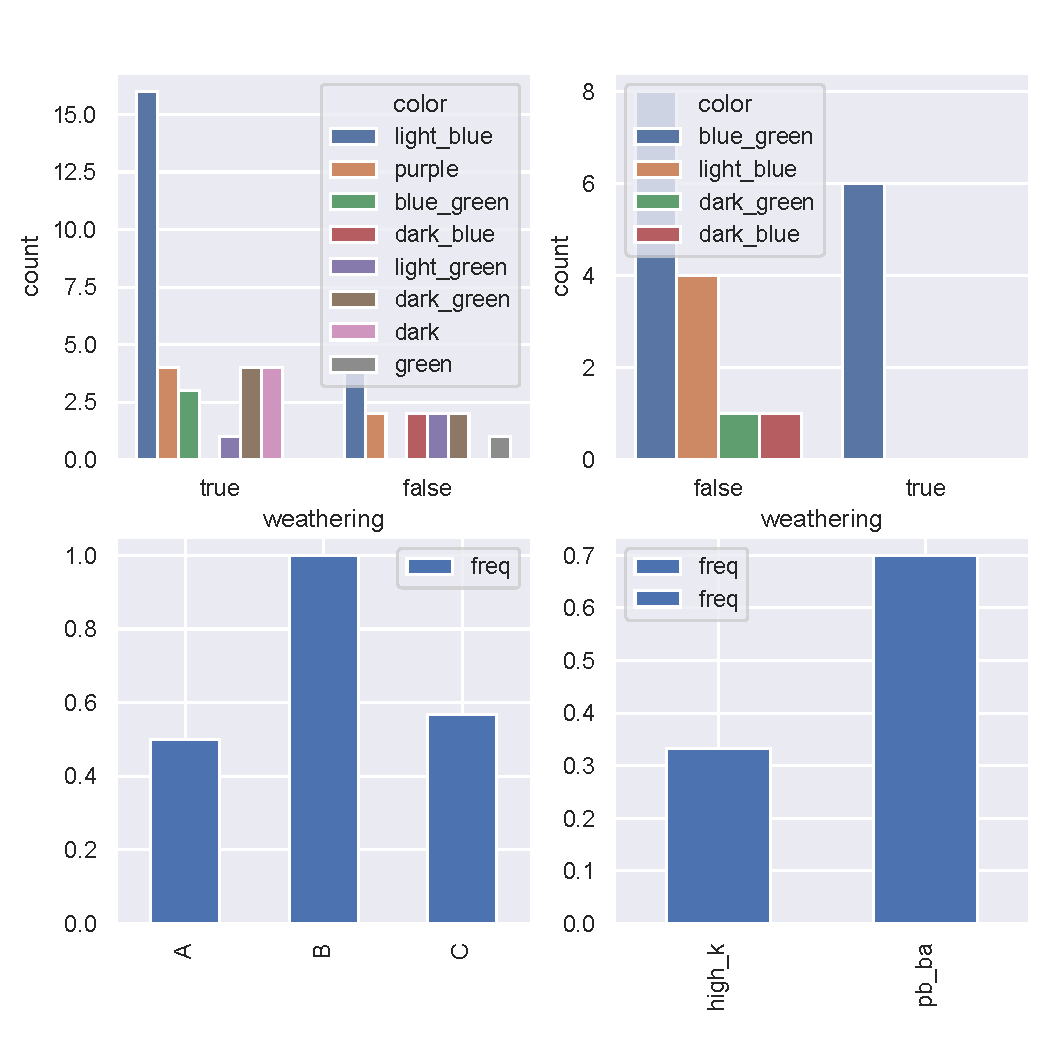
\includegraphics[width=.9\textwidth]{physical_weathering.pdf}
    \caption{物理特征与风化的关系}
    \label{bb}
\end{figure}


\subsection{风化化学成分的选择}

为了判断风化对化学成分含量的影响,
我们对不同玻璃风化前后元素含量的均值进行分析,
发现风化前后的均值有一定差别,
但由于文物风化受诸多因素的影响,无论是添加的助燃剂不同,
检测化学成分的误差,还是埋藏的环境不同,
都可能导致同一种玻璃的各个化学成分有很大的差别,
因此我们引入方差分析寻找风化和化学成分之间的相关性,
筛选出合适的风化化学成分并探究其统计规律。

\subsubsection{使用独立样本$t$检验进行方差分析}
常见的相关性分析方法通常对变量有一定要求,
如皮尔逊相关系数需要两个变量是连续数据且呈正态分布,
或接近正态分布的单峰分布,并不适用于我们研究的类别变量
斯皮尔曼相关系数要求两个变量一个变量为定序数据,
另一个为定距数据,或两个变量均为非正态分布的定距数据,
同样也不符合我们的要求;
最终,我们选择独立样本$t$检验来验证相关性。

独立样本$t$检验,适用于两个变量为定类数据和定量数据的情况,
它可以帮助我们判断同种玻璃的不同种化学成分是否在风化前后有显著变化,
减少了前文提到的可能存在误差和影响,
让我们选择的风化化学成分更加合理、具有说服力。

文物是否风化,可能受到多种化学成分的影响,
但我们假设各化学成分之间没有交互作用,
且我们的数据是连续的、呈正态分布的。在独立样本$t$检验中,
我们首先假设同种玻璃的某种物质风化前后的均值相等,这个零假设可以表示为

\begin{equation}
    H_0: \mu_{1} = \mu_{2}
\end{equation}

其中$\mu_{1}$为风化前某化学元素含量的均值,
$\mu_{2}$为风化后某化学元素含量的均值。

根据零假设和当前样本,计算$t$值,其公式为

\begin{equation}
    t = \dfrac{\bar{x} - \bar{y}}{\sqrt{\dfrac{s^2_1}{n_1} + \dfrac{s^2_2}{n_2}}}
\end{equation}

其中$\bar{x}$,$\bar{y}$为两种玻璃样本的某化学元素含量均值,
$s_1$,$s_2$是两种玻璃样本的某化学元素含量标准差,
$n_1$,$n_2$为两种玻璃的样本数量。
接着,为了获取数据集中可以自由变化的值的数量,我们计算自由度$af$,由于我们有两个样本集,所以公式应该如下所示:
\begin{equation}
    af=n_1 +n_2 - 2
\end{equation}

对于alpha level,为了在I型错误和II型错误中达到良好平衡,
我们令$\alpha=0.05$
结合alpha level $\alpha$ 和自由度$af$,
我们在双尾$T$分布表中可以查到$p$的值,
若$p$的值小于0.05,则我们拒绝零假设,即该化学成分与风化相关。
通过计算我们得到表\ref{p-value-table}。

\begin{table}[h]
    \begin{subtable}[h]{0.45\textwidth}
        \centering
        \begin{tabular}{cc|cc}
            \toprule[1.5pt]
            化学成分          & p-value & 化学成分          & p-value \\
            \midrule[1pt]
            \chemfig{SiO_2}   & 0.0000  & \chemfig{Na_2O}   & 0.1098  \\
            \chemfig{K_2O}    & 0.0000  & \chemfig{CaO}     & 0.0187  \\
            \chemfig{MgO}     & 0.0052  & \chemfig{Al_2O_3} & 0.0058  \\
            \chemfig{Fe_2O_3} & 0.0293  & \chemfig{CuO}     & 0.3260  \\
            \chemfig{PbO}     & 0.1116  & \chemfig{BaO}     & 0.1998  \\
            \chemfig{P_2O_5}  & 0.1162  & \chemfig{SrO}     & 0.0836  \\
            \chemfig{SnO_2}   & 0.5274  & \chemfig{SO_2}    & 0.2443  \\
            \bottomrule[1.5pt]
        \end{tabular}
        \caption{高钾玻璃}
    \end{subtable}
    \hfill
    \begin{subtable}[h]{0.45\textwidth}
        \centering
        \begin{tabular}{cc|cc}
            \toprule[1.5pt]
            化学成分          & p-value & 化学成分          & p-value \\
            \midrule[1pt]
            \chemfig{SiO_2}   & 0.0009  & \chemfig{Na_2O}   & 0.6612  \\
            \chemfig{K_2O}    & 0.2074  & \chemfig{CaO}     & 0.0544  \\
            \chemfig{MgO}     & 0.3332  & \chemfig{Al_2O_3} & 0.6107  \\
            \chemfig{Fe_2O_3} & 0.2024  & \chemfig{CuO}     & 0.5690  \\
            \chemfig{PbO}     & 0.0055  & \chemfig{BaO}     & 0.8747  \\
            \chemfig{P_2O_5}  & 0.0126  & \chemfig{SrO}     & 0.4165  \\
            \chemfig{SnO_2}   & 0.2602  & \chemfig{SO_2}    & 0.4473  \\
            \bottomrule[1.5pt]
        \end{tabular}
        \caption{铅钡玻璃}
    \end{subtable}
    \caption{是否风化和各个化学成分之间的关系}
    \label{p-value-table}
\end{table}



\subsubsection{风化化学成分及其统计规律}

根据独立样本$t$检验给出的结果,和同种玻璃风化前后不同化学成分的均值对比图表,
我们可知对于高钾玻璃而言,
\chemfig{SiO_2}、\chemfig{K_2O}、\chemfig{CaO}、\chemfig{MgO}和\chemfig{Al_2O_3}是风化化学成分,
其统计学规律为\chemfig{SiO_2}在风化后含量上涨,
\chemfig{K_2O}、\chemfig{CaO}、\chemfig{MgO}和\chemfig{Al_2O_3}在风化后含量下降;
对铅钡玻璃而言\chemfig{SiO_2}、\chemfig{Fe_2O_3},
\chemfig{PbO}和\chemfig{P_2O_5}是主要风化化学成分,
其统计学规律为\chemfig{SiO_2}和\chemfig{Fe_2O_3}在风化后含量下降,
\chemfig{PbO}和\chemfig{P_2O_5}在风化后含量上涨。

\subsection{预测风化前化学成分含量的模型}

在上一问中,我们针对不同种类的玻璃分别提取了风化化学成分,
这些化学成分在风化前后其含量发生了显著变化,
所以在我们构建预测风化前化学成分含量的模型时,
我们假设除了风化化学成分以外的其他化学成分所占百分比不会发生改变。

通过独立样本$t$检验,
我们知道这些风化化学成分的均值是有很大变化且有统计学意义的,
因此我们设定变化量$\Delta$:

\begin{equation}
    \Delta_{i} = p_{\left (i,\text{after}\right )} - p_{\left (i,\text{before}\right )}
\end{equation}

其中$i$代表某种化学成分,$p$为均值。
基于此,我们构建风化前化学成分含量的预测模型

\begin{equation}
    y = p_{\left ( i,\text{after} \right ) }+\Delta _{i} = 2p_{\left ( i,\text{after} \right ) }-p_{\left ( i,\text{before} \right )}
\end{equation}

The Corning Archaeological Reference Glasses(康宁标准)
是一种被广泛用作考古和历史玻璃的化学分析标准,
它们的成分接近古代玻璃的主要类型。
结合康宁标准和多篇文献的化学成分分析结果,
我们归纳数据,得到了这些风化化学成分在未风化玻璃文物中的含量取值范围。
我们的预测模型所得出的数据,基本落在这个区间范围内。
因此我们认为该模型是符合实际的。


\section{问题二的建模与求解}

为了对两种类型的玻璃进行亚类划分,
我们采用非监督学习$K$-means\cite{hartigan1979algorithm}聚类算法,
将相似的数据样本分为一组,进行数据标注。
随后我们使用已经完成的标注的数据训练决策树,
得到可解释性较强的分类依据。

\subsection{两种玻璃类型的分类规律}


\subsubsection{通过化学特征分类}
对于两种玻璃类型的分类规律,
我们绘制了不同种玻璃之间同种化学成分的箱型图,共14张,
我们筛选出了5张更具意义的箱型图(图 \ref{fig:chemical_material_box_plot}),
并认为其是具有主要分类意义的化学成分。

\begin{figure}[!h]
    \centering
    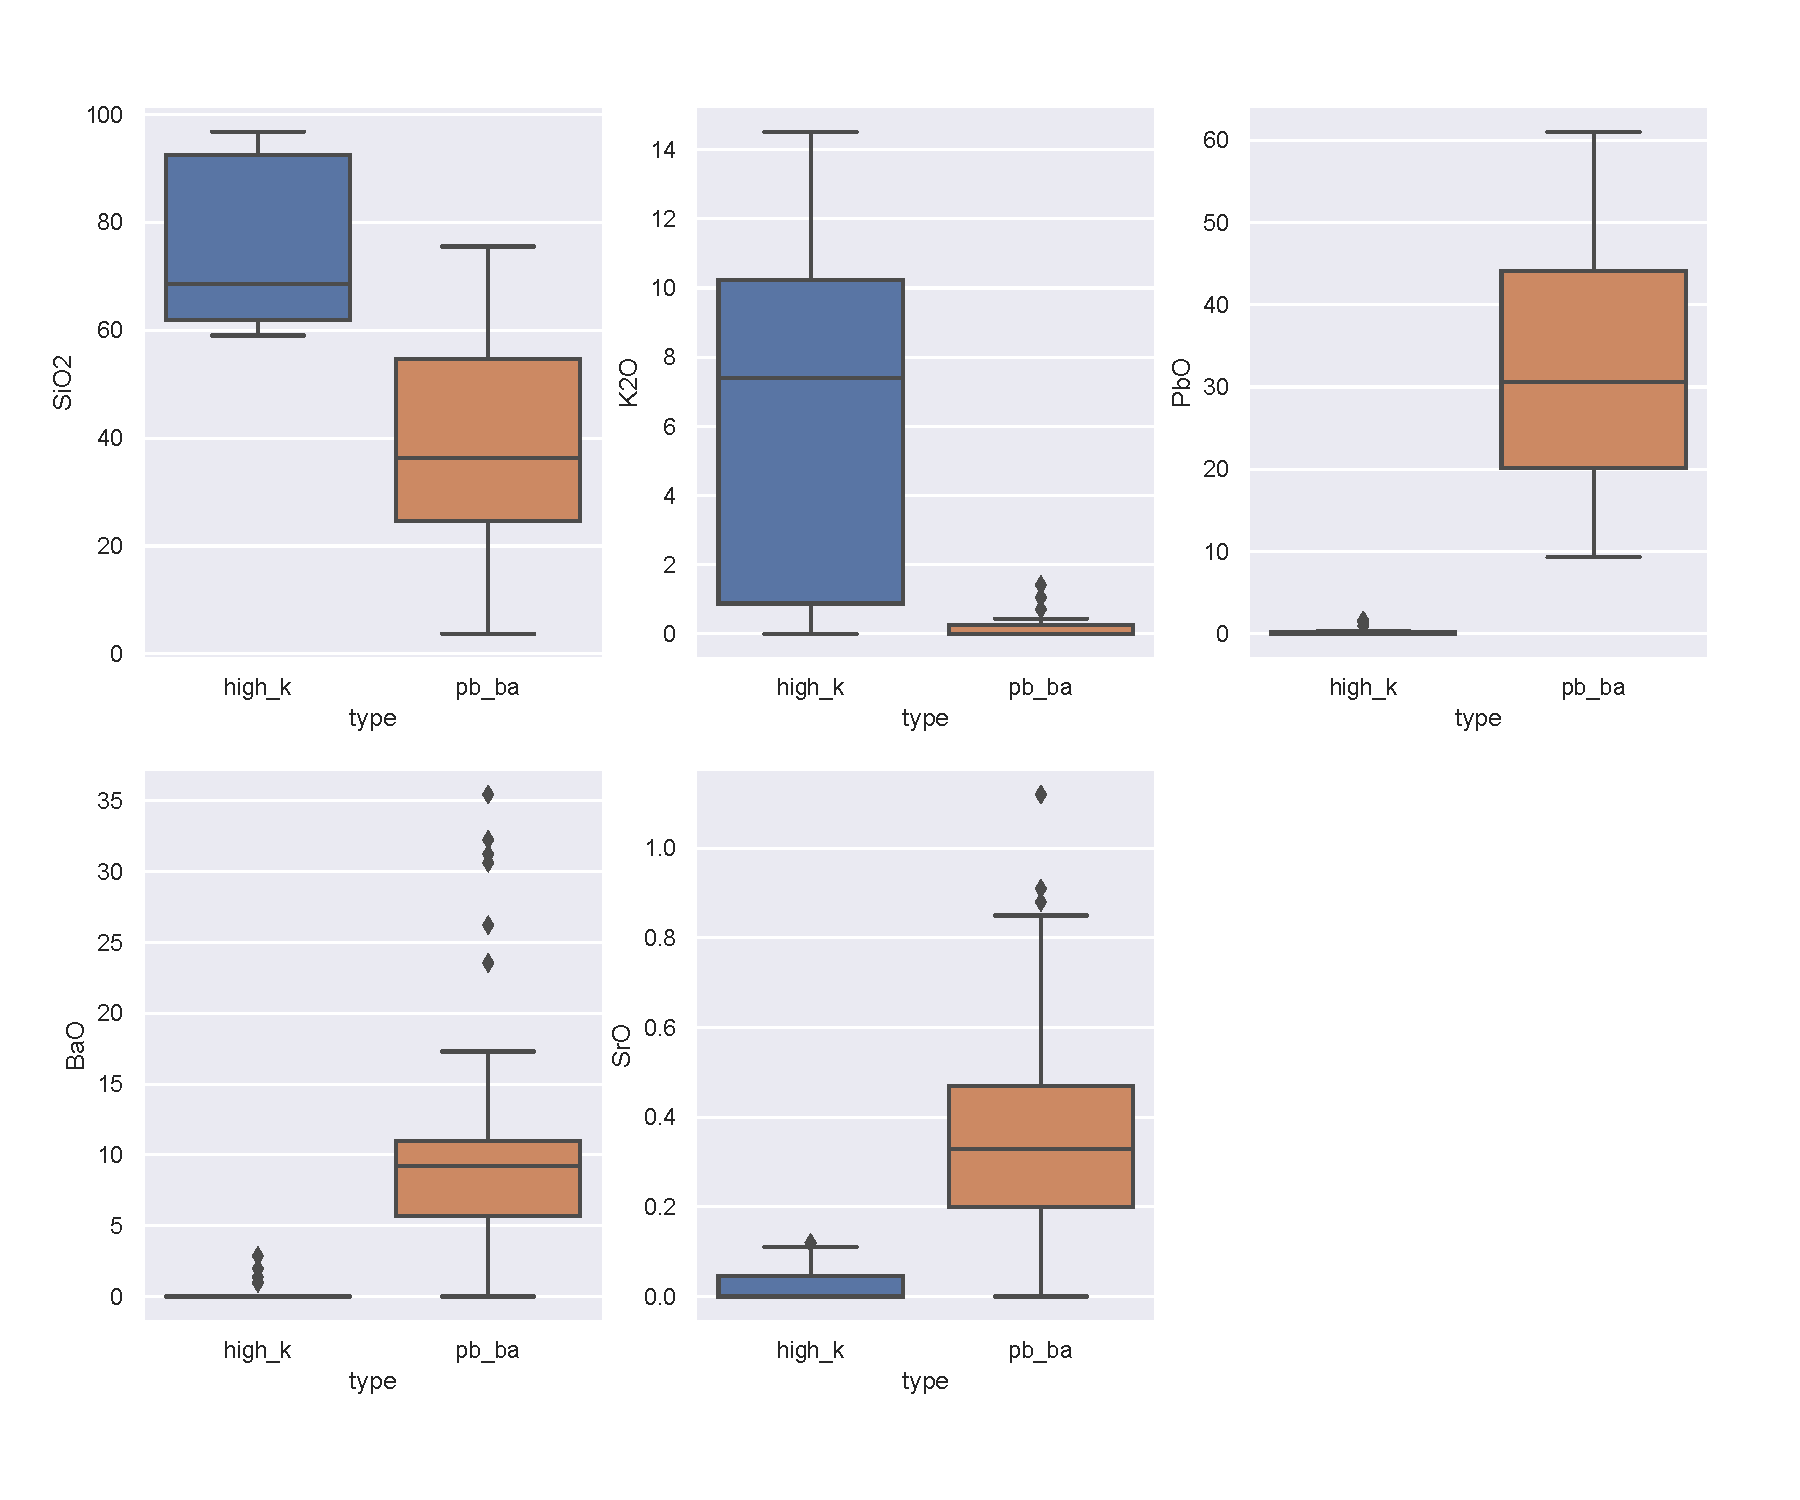
\includegraphics[width=.9\textwidth]{five_main_material.pdf}
    \caption{不同种玻璃之间同种化学成分的箱型图}
    \label{fig:chemical_material_box_plot}
\end{figure}

其中,\chemfig{PbO}可以极好的区分两种玻璃类型。
两种玻璃类型的箱型图没有重合部分,
且高钾玻璃的离群值也没有与铅钡玻璃冲突,
因此我们可以认为,\chemfig{PbO}的含量多少是两种玻璃类型分类的一大重要分类规律。

\subsubsection{通过物理特征分类}
如上文所述,在铅钡玻璃的样本中,
出现的纹饰只有A和C,纹饰B只有在高钾玻璃种才出现,
所以我们也可以通过判断纹饰类别来区分两种玻璃类型。
虽然有关铅钡玻璃的样本数量不够庞大,无法断定铅钡玻璃一定无样式B,
但铅钡玻璃的样本数量相对而言大于高钾玻璃的样本数量,
所以我们可以初步认为通过纹饰B的有无来区分两种玻璃类型。

\subsection{数据预处理以及特征工程}

\subsubsection{特征提取}
由前文可知,有5种化学成分对玻璃类别的分类存在重要影响,
分别为\chemfig{SiO_2}, \chemfig{K_2O},\chemfig{PbO},\chemfig{BaO} ,\chemfig{SrO}
为了降低数据的维度并且降低噪声的干扰,
我们选取上述的5个特征参与后续训练,
根据题意,在亚类划分时当前玻璃的类别已知,
故玻璃类别也作为特征参与训练。

\subsubsection{数据标准化}
在训练之前,我们使用z-score对数据进行标准化,
将数据缩放到特定的范围内,
以提升模型的收敛速度和精度。
\begin{equation}
    x = \dfrac{x - \mu}{\sigma}
\end{equation}

其中$\mu$ 为均值,$\sigma$为标准差


\subsection{聚类数量模型}
在$K$-means聚类算法中,选择不同的簇类数量$k$,
对聚类的准确性有较大响,
考虑到当前聚类任务中``基准真相''(Ground truth) 未知,
因此我们引入David L. Davies 和 Donald W. Bouldin
于 1979 年提出的聚类算法评估的指标
Davies-Bouldin Index (DBI) \cite{davies1979cluster}
对参数$k$进行搜索以确定最佳的$k$值。


\begin{table}[!htbp]
    \centering
    \setstretch{1.1}
    \begin{tabular}{cc|cc}
        \toprule[1.5pt]
        符号     & 说明                              & 符号     & 说明                            \\
        \midrule[1pt]
        $C_{i}$  & 聚类$i$                           & $T_{i}$  & 聚类$i$中数据点的个数           \\
        $X_{ij}$ & 聚类$C_{i}$中第$j$个数据点        & $A_{i}$  & 聚类$i$的质心                   \\
        $N$      & 聚类总数量                        & $S_{i}$  & 聚类$i$的聚类半径               \\
        $M_{ij}$ & 聚类 $C_i$ 和 $C_j$之间的分离度量 & $R_{ij}$ & 聚类 $C_i$ 和 $C_j$之间的相似度 \\
        \bottomrule[1.5pt]
    \end{tabular}
    \caption{聚类评判指标符号表}\label{tab:clust_judge}
\end{table}

\subsubsection{聚类半径}


我们定义$S_{i}$表示聚类$C_{i}$内部的紧凑程度,即聚类半径

\begin{equation}
    S_{i} = \left \{ \dfrac{1}{T_{i}}  \sum_{j=1}^{T_{i}} \left | X_{ij} - A_{i} \right |^{q}  \right \}^{1/q}
\end{equation}

其中,当$q = 1$时,$S_i$表示各个样本点到质心距离的均值,
当$q = 2$时,$S_i$是各个样本点到质心距离的标准差。
$S_{i}$ 越大则聚类半径越大,集群内部越分散,
$S_{i}$ 越小则聚类半径越小,集群内部越集中。


\subsubsection{聚类间分离度量}
我们定义$M_{ij}$为集群$C_{i}$和${C_j}$之间的分离度量:


\begin{equation}
    M_{ij} = \left \{ \sum_{k=1}^{N} \left | a_{ki} - a_{kj} \right |^{p}  \right \} ^{1/p}
\end{equation}

其中,$a_{ki}$ 表示$C_{i}$的质心的第$k$个属性的值。
当$p = 1$时,使用曼哈顿距离衡量质心间距离,
当$p = 2$时,使用欧几里得距离衡量质心间距离。
$M_{ij}$ 越大则聚类$ij$分离程度越好,
越小则聚类$ij$分离程度越差。


\subsubsection{聚类间相似度}
为了度量聚类方案好坏,我们引入$R_{ij}$表示$C_i$ 和 $C_j$ 之间的相似度
\begin{equation}
        R_{ij} = \dfrac{S_i + S_j}{M_{ij}}
\end{equation}

当聚类半径极小,聚类间分离度量极大时,
我们认为两个聚类之间的相似度小,
即$R_{ij}$越小则聚类间相似度越小,反之亦然。

\subsubsection{Davies-Bouldin 指数}

我们定义:
\begin{gather}
        D_{i}  = \displaystyle\max_{i \neq j} R_{ij}                       \\
        DB     = \dfrac{1}{k} \displaystyle\sum_{i=1}^k D_{k}
\end{gather}

$D_i$表示聚类$C_i$与其他聚类相似度最大的情况,
并使用$D_i$计算所有聚类的最大相似度的均值,
最终得到Davies-Bouldin指数,
该指数越小则表示当前聚类算法表现越良好,
因此,我们将$DB$作为目标函数,寻找最优的聚类个数$N$,
使得聚类效果最好。

\begin{equation} \label{eq:best_n_cluster}
    \underset{N}{\mathrm{argmin}} \dfrac{1}{N} \displaystyle\sum_{i=1}^{N} D_{i} \quad N \in 1, 2 \cdots 10
\end{equation}

我们使用sklearn\cite{scikit-learn}求解(\ref{eq:best_n_cluster})得到最佳聚类个数为$N = 5$



\subsection{玻璃亚类划分模型}
在确定了最佳$k$值为5之后,我们根据选取的五个特征,
通过优化目标函数(\ref{eq:k-means})的方式,对玻璃类型进行亚类划分,

\begin{equation}\label{eq:k-means}
    inertia = \sum_{i=0}^{n} \min_{\mu_{j}}\left ( \left | x_{i}-\mu _{j} \right | ^{2} \right )
\end{equation}
其中$\mu_{j}$是聚类$j$的均值,即质心,$x_i$为待分类的数据点。
我们用以下方法对聚类进行划分:
\begin{enumerate}
    \item 在所有样本点中随机选取5个样本点作为聚类中心。
    \item 计算每个样本点到不同簇类中心的距离$d$,并将该样本点划分给$d$值最小的聚类。
    \item 重新计算聚类中心。
    \item 不断迭代第2、3步,直到聚类中心不再改变。
\end{enumerate}

我们选取上文所述的5个主要的化学成分和玻璃类型作为特征,
使用sklearn \cite{scikit-learn} 训练模型,
最终我们将高钾玻璃分为2类,将铅钡玻璃分为3类,
并对数据进行标注,得到了“亚类”的特征。

在完成了数据标注的工作后,
考虑到决策树的可解释性好的特点,
我们将数据划分为训练集(60\%)和验证集(40\%),
使用sklearn \cite{scikit-learn} 训练模型,
并对超参数进行搜索,限制其最大深度,
保证决策树的决策方案尽可能简单,最终我们得到表\ref{tab:sub_class_judge} 和图\ref{fig:decision_tree}

\begin{table}[!htbp]
    \centering
    \setstretch{1.1}
    \begin{tabular}{c|c}
        \toprule[1.5pt]
        亚类   & 分类依据 \\
        \midrule[1pt]
        铅钡-0 & $ \chemfig{PbO} \leqslant 33.55$ 且 $ 41.19 < \chemfig{SiO_2} \leqslant 41.19 $ 且 $\chemfig{K_2O} \leqslant 3.99$\\
        铅钡-1 & $ \chemfig{PbO} > 33.55$ \\
        高钾-2 & $ \chemfig{PbO} \leqslant 33.55$ 且 $ 41. 19 < \chemfig{SiO_2} \leqslant 73.195 $ 且 $\chemfig{K_2O} > 3.99$ \\
        高钾-3 & $ \chemfig{PbO} \leqslant 33.55$ 且 $\chemfig{SiO_2} \geqslant 73.195 $ \\
        铅钡-4 & $ \chemfig{PbO} \leqslant 33.55$ 且 $\chemfig{SiO_2} \leqslant 41.19 $ \\
        \bottomrule[1.5pt]
    \end{tabular}
    \caption{玻璃亚类分类依据}\label{tab:sub_class_judge}
\end{table}

\begin{figure}[!h]
    \centering
    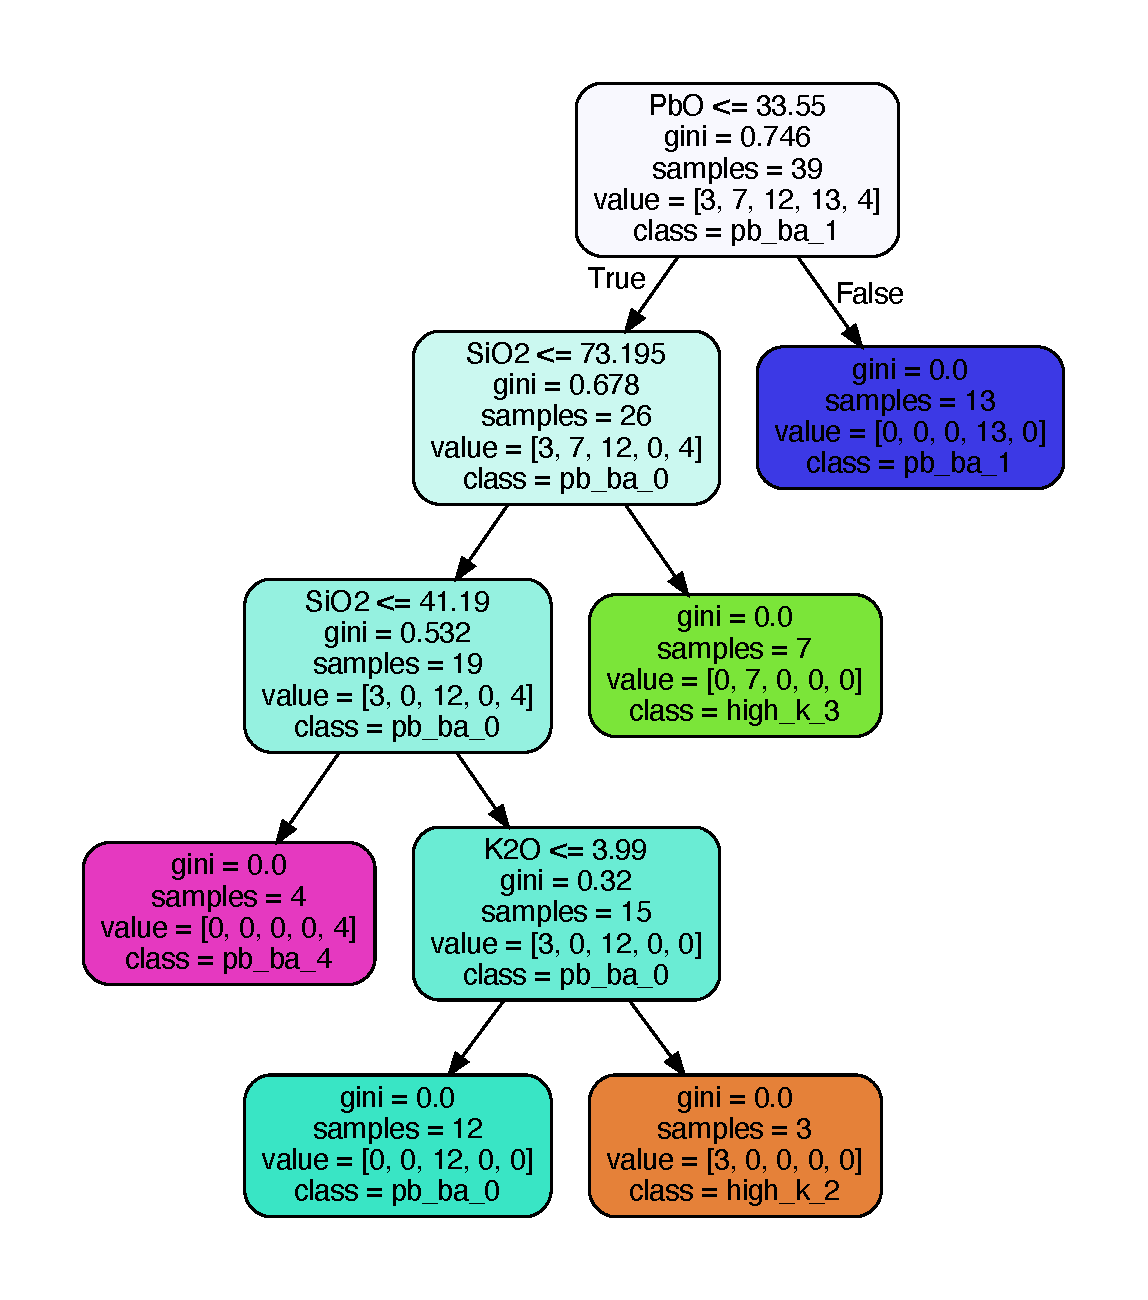
\includegraphics[width=.6\textwidth]{decision_tree.pdf}
    \caption{决策树}
    \label{fig:decision_tree}
\end{figure}





\subsection{模型评估}
对于分类问题,通常使用 ROC (Receiver operating characteristic) \cite{fawcett2006introduction}
曲线比较评估分类器,ROC 曲线由 FPR(假阳率) 作为$x$ 轴,
TPR(真阳率)作为$y$ 轴组成,与之对应的,AUC (Area Under the Curve) \cite{fawcett2006introduction},
即 ROC 曲线下面积,常用来定量衡量二元分类器的性能,一个分类器的 AUC 值
越接近于 1, 则说明其越接近于完美分类器。

本文使用的分类属于多元分类器,对于多元分类器的 ROC 曲线的绘制,
我们定义 $C$ 为所有类别的集合,第 $i$ 个 ROC 曲线分别使用 $c_i \in C$
作为阳性类(positive class),剩余的类作为一类即阴性类(negative class)即
\begin{gather}
    P_i = c_i  \\
    N_i = \bigcup_{j \neq i} c_j \in C
\end{gather}

对于多元分类器的AUC值,通常有两种计算方式:
\begin{equation}
    \text{AUC} = \sum_{c_i \in C} \text{AUC}(c_i) \cdot p(c_i)
\end{equation}

其中$p(c_i)$ 为$c_i$ 在 $C$ 中的权重

\begin{equation}
    \text{AUC} = \dfrac{2}{\left | C \right |\left ( \left | C \right |-1  \right )}\sum_{\left \{ c_{i},c_{j}\in C \right \} }\text{AUC}\left ( c_{i},c_{j} \right )
\end{equation}

其中$\text{AUC}(c_j, c_j)$ 表示将$c_j, c_i$ 作为二分类标签的AUC值
如图(\ref{fig:decision_tree_roc_auc})所示,两种评估标准下分类器的AUC值均接近于$1$,即接近完美分类器的性能。

\begin{figure}[!h]
    \centering
    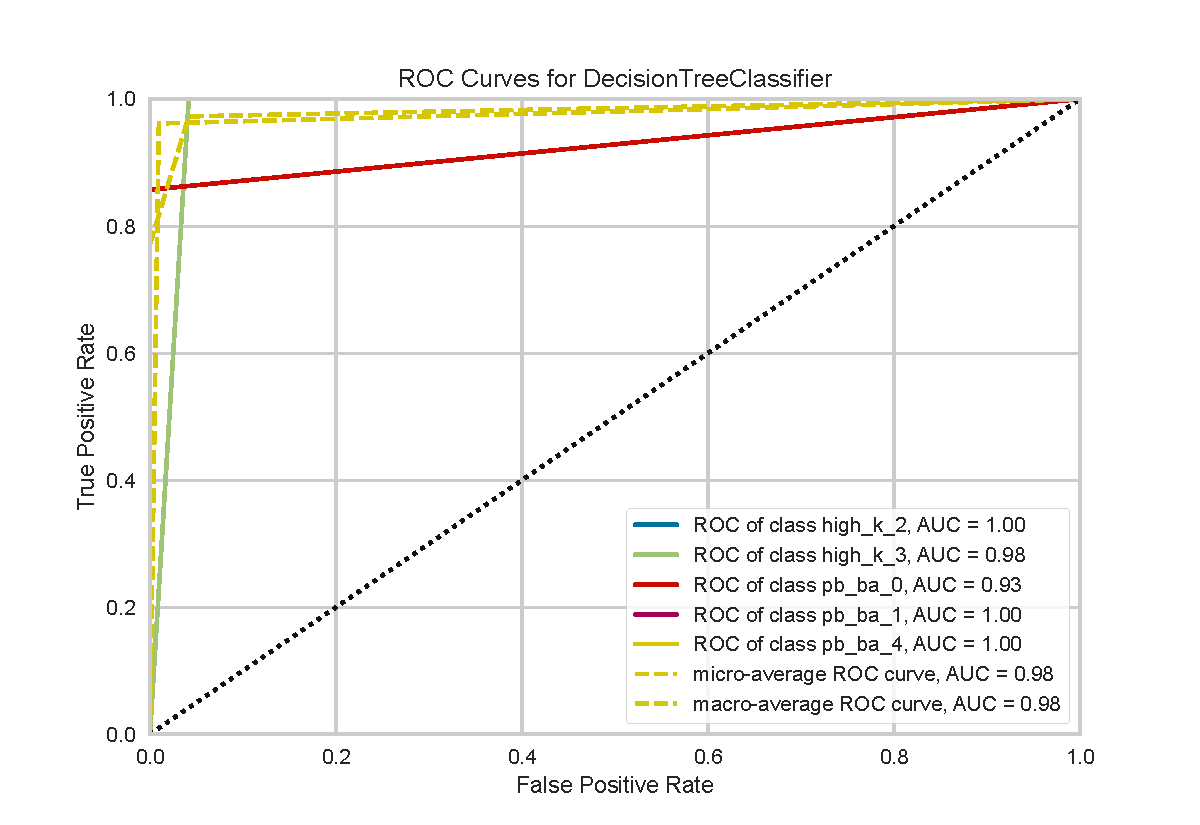
\includegraphics[width=.9\textwidth]{decision_tree_roc_auc.pdf}
    \caption{决策树的ROC-AUC曲线}
    \label{fig:decision_tree_roc_auc} 
\end{figure}




\section{问题三的建模与求解}
 
\subsection{未知类别玻璃文物的亚类划分}
根据问题二中所训练的决策树模型,
对表单三的文物进行预测,
判断每个文物所属亚类。


\subsubsection{数据预处理}
将附件``表单三''中的各个文物样本,
使用和前文相同的方式进行数据预处理
并根据上文的结论选取\chemfig{SiO_2}, \chemfig{K_2O},\chemfig{PbO},\chemfig{BaO} ,\chemfig{SrO}
含量作为特征参与训练

\subsubsection{玻璃类别的划分}
考虑到问题二中的决策树模型
使用了玻璃类别对玻璃亚类进行预测,
表单三中的数据并没有提供这部分信息,
故我们先对玻璃类别进行预测,
根据前文所述,\chemfig{PbO}含量是决定玻璃类别的重要指标,
故我们使用\chemfig{PbO}含量对玻璃类别进行简单的划分。


\subsubsection{玻璃亚类的预测}
基于上述的划分结果,我们使用问题二中得到的模型
对扩展后的特征进行训练,最终得到的结果为,
亚类为high\_k\_3的玻璃文物有3件;
亚类为pb\_ba\_0的玻璃文物有2件;
亚类为pb\_ba\_1的玻璃文物有2件;
亚类为pb\_ba\_4的玻璃文物有1件;
详细分类结果见表\ref{tab:classify_result}。

\begin{table}[!htbp]
    \centering
    \begin{tabular}{cccccccc}
        \toprule[1.5pt]
        文物编号 & 预测玻璃类型 & 预测玻璃亚类 & \chemfig{PbO} & \chemfig{SiO_2} & \chemfig{K_2O} & \chemfig{BaO} & \chemfig{SrO} \\
        \midrule[1pt]
        A1       & high\_k      & high\_k\_3   & 0.00          & 78.45           & 0.00           & 0.00          & 0.03          \\
        A2       & pb\_ba       & pb\_ba\_1    & 34.30         & 37.75           & 0.00           & 0.00          & 0.00          \\
        A3       & pb\_ba       & pb\_ba\_1    & 39.58         & 31.95           & 1.36           & 4.69          & 0.52          \\
        A4       & pb\_ba       & pb\_ba\_4    & 24.28         & 35.47           & 0.79           & 8.31          & 0.28          \\
        A5       & pb\_ba       & pb\_ba\_0    & 12.23         & 64.29           & 0.37           & 2.16          & 0.21          \\
        A6       & high\_k      & high\_k\_3   & 0.00          & 93.17           & 1.35           & 0.00          & 0.00          \\
        A7       & high\_k      & high\_k\_3   & 0.00          & 90.83           & 0.98           & 0.00          & 0.00          \\
        A8       & pb\_ba       & pb\_ba\_0    & 21.24         & 51.12           & 0.23           & 11.34         & 0.31          \\
        \bottomrule[1.5pt]
    \end{tabular}
    \caption{分类结果}\label{tab:classify_result} \centering
\end{table}


\subsection{模型的敏感性分析}
为了验证我们的模型的鲁棒性,
我们对决策树进行敏感性分析,
我们以前文的预测结果作为baseline,
在一定范围内改变\chemfig{SiO_2}, \chemfig{K_2O},\chemfig{PbO},\chemfig{BaO} ,\chemfig{SrO}
我们记为随机扰动$\Delta x$,
并使用决策树再次预测其所属玻璃亚类,记为disturbance
当随机扰动导致预测结果发生变化时,即 baseline $\neq$ disturbance时,
停止基于随机扰动。并记下此时的$\Delta x$

考虑到决策树中只使用了\chemfig{SiO_2}, \chemfig{K_2O}, \chemfig{PbO}
进行预测,我们只针对这三种元素给予随机扰动(每次仅改变一个元素的含量),
我们得到:

\begin{itemize}
    \item 对于\chemfig{SiO_2}的随机扰动$ -7\% \leqslant \Delta x \leqslant 14\% $,随机扰动不会影响预测值
    \item 对于\chemfig{K_2O}的随机扰动$ -99\% \leqslant \Delta x \leqslant 980\% $,随机扰动不会影响预测值
    \item 对于\chemfig{PbO}的随机扰动$ 2.7\% \leqslant \Delta x \leqslant 39\% $,随机扰动不会影响预测值
\end{itemize}

即在其他化学成分含量不变的情况下,
当\chemfig{SiO_2}的增加14\%,会对模型产生影响;
当PbO增加39\%时,会对模型产生影响。当\chemfig{K_2O}增加980\%时,
会对模型产生影响。
当\chemfig{SiO_2}的减少7\%时,会对模型产生影响;当PbO减少2.7\%, 
会对模型产生影响。所以我们可得出再增加化学成分含量时,\chemfig{SiO_2}比\chemfig{PbO}对模型的影响程度更大。
在减少的情况下,\chemfig{PbO}比\chemfig{SiO_2}对模型的影响程度更大。模型对\chemfig{K_2O}的几乎不敏感。

\section{问题四的建模与求解}
\subsection{同种玻璃中化学成分之间的关联关系}

为了探究同种玻璃之间化学成分的关联关系,
我们选取了\chemfig{K_2O},\chemfig{SiO_2},\chemfig{SiO_2}, \chemfig{SrO},\chemfig{PbO}, \chemfig{BaO}五种化学成分,
针对不同种玻璃,分别进行散点图绘制。
 
\subsubsection{高钾玻璃中化学成分之间的关联关系}

在铅钡玻璃中,两两化学成分结合所绘制的散点图如图(\ref{aa}),我们可以得到以下关联关系:
\begin{figure}[!h]
    \centering
    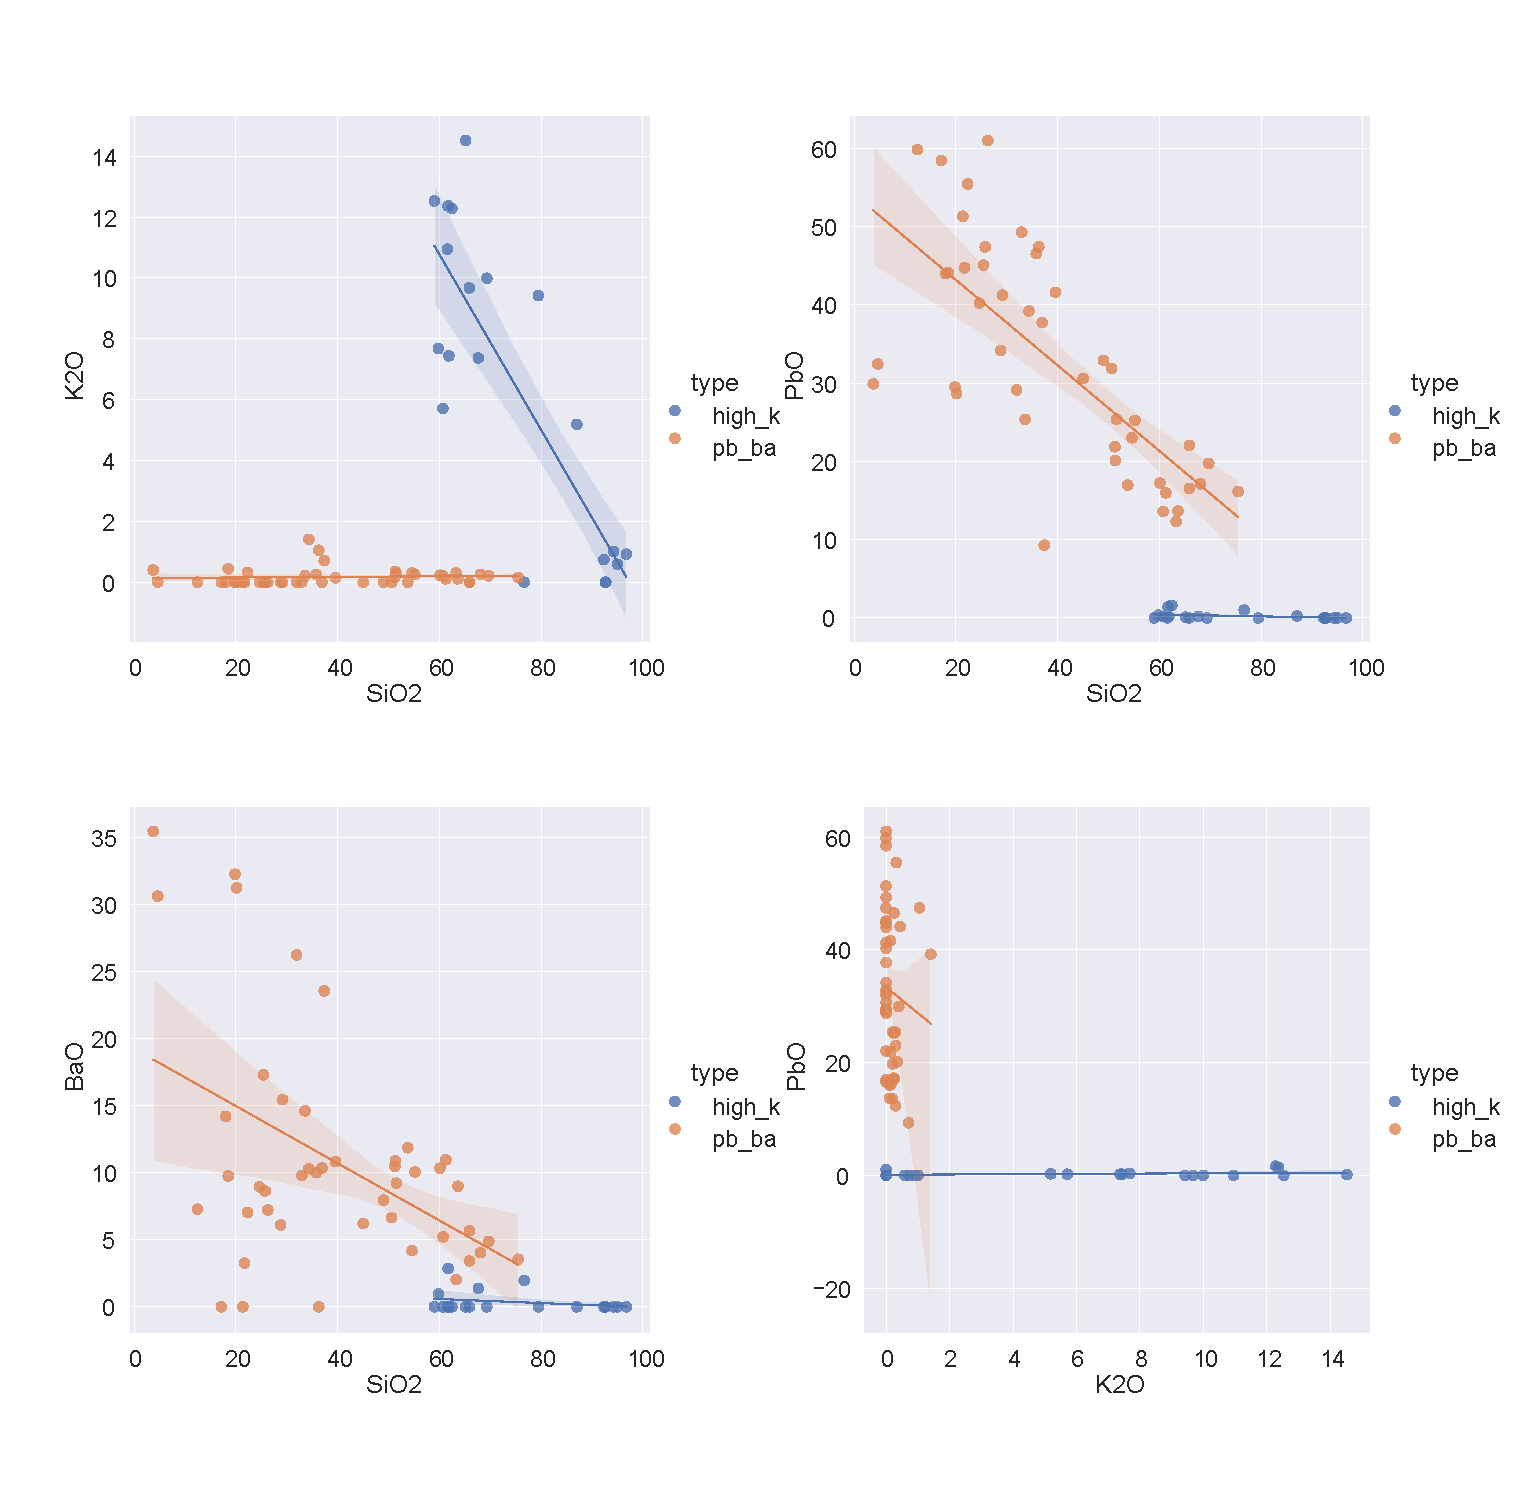
\includegraphics[width=.9\textwidth]{aa.pdf}
    \caption{化学成分关联关系图}
    \label{aa}
\end{figure}


\begin{itemize}
    \item \chemfig{SiO_2{-}K_2O}之间的关联关系较强,它呈负相关关系,即当\chemfig{SiO_2}的占比增多时,\chemfig{K_2O}的占比就会减少;对于该直线而言,它的残差相对较小。

    \item 以\chemfig{SiO_2}作为$x$轴,其他化学成分作为$y$轴的散点图,其关联关系都为负相关关系,但数据点过于分散,拟合的直线残差过大,但相对而言有一个主要趋势。

    \item 散点图\chemfig{K_2O{-}PbO},它的离群点相对而言较少,其关系呈正相关,即当\chemfig{K_2O}的占比增多时,\chemfig{PbO}的占比也相应增加。
\end{itemize}
       
\subsubsection{铅钡玻璃中化学成分之间的关联关系}

在铅钡玻璃中,两两化学成分结合所绘制的散点图如图(\ref{aa}),我们可以得到以下关联关系:
\begin{itemize}
    \item \chemfig{SiO_2{-}K_2O}的散点图呈正相关;
    \item \chemfig{SiO_2{-}PbO}和\chemfig{SiO_2{-}BaO}的散点图呈负相关,样本点大多数都沿着直线分布,残差较小。 
    \item 以\chemfig{K_2O}作为横坐标,\chemfig{PbO}作为纵坐标的散点图,
其主要呈负相关关系,但残差较大。
\end{itemize}

 
\subsection{不同种玻璃中化学成分关联关系的差异性}
1. 在高钾玻璃中,\chemfig{SiO_2}和\chemfig{K_2O}呈负相关关系;
而在铅钡玻璃中,\chemfig{SiO_2}和\chemfig{K_2O}呈正相关关系。

2. 在高钾玻璃中,\chemfig{K_2O}和\chemfig{PbO}呈正相关关系;
而在铅钡玻璃中,\chemfig{K_2O}和\chemfig{PbO}呈负相关关系。


\section{模型评价}
\subsection{模型优点}
\begin{enumerate}
    \item 在聚类数量模型中,我们使用Davies-Bouldin Index (DBI) 对参数 $k$ 进行搜索以确定最佳的 $k$ 值。找到最佳的聚类个数,准确性更高。
    \item 使用决策树进行亚类划分,并使用多元分类器的AUC值衡量分类器的性能,AUC值接近完美模型,得到的划分结果的合理性高。
    \item 决策树的深度浅,分枝少,得到的分类依据更具有可解释性。
\end{enumerate}
\subsection{模型缺点}
\begin{enumerate}
    \item 对于玻璃亚类划分模型,通过$K$-means算法对不同类别的玻璃按照合适的化学成分进行亚类划分。但是由于$K$-means的使用对于初始的簇中心敏感,不同的选取方式会得到不同的结果。
    \item 使用决策树对于玻璃亚类分类提供依据,但是对于各类别样本数量不一致,进行属性划分时,不同的判定准则可能会带来不同的划分趋向。也容易忽略数据集中属性的相关关系。
\end{enumerate}


% Reference

%\phantom{\cite{ramalho2022fluent}}
%\phantom{\cite{mckinney2012python}}
%\phantom{\cite{scikit-learn}}
%\phantom{\cite{reback2020pandas}}
%\phantom{\cite{harris2020array}}
%\phantom{\cite{Hunter2007}}
%\phantom{\cite{Waskom2021}}
%\phantom{\cite{bengfort_yellowbrick_2018}}

\nocite{*}
\bibliographystyle{gbt7714-numerical}
\bibliography{ref}


\newpage

\newpage

%附录
\begin{appendices}
\section{数据预处理}

\begin{lstlisting}[language=python]
import pandas as pd
df1 = pd.read_excel("../data_source/data.xlsx", sheet_name="表单1")
df2 = pd.read_excel("../data_source/data.xlsx", sheet_name="表单2")
df3 = pd.read_excel("../data_source/data.xlsx", sheet_name="表单3")
df1.isnull().sum()
df1.rename(columns={'文物编号': "id", '纹饰': "pattern", '类型': "type", '颜色': 'color', '表面风化': 'weathering'}, inplace=True)
df2.isnull().sum()
df2.fillna(0, inplace=True)
df2.rename(columns={
    '文物采样点' : "sample_place",
    '二氧化硅(SiO2)': "SiO2",
    '氧化钠(Na2O)' : "Na2O",
    '氧化钾(K2O)': "K2O",
    '氧化钙(CaO)': "CaO",
    '氧化镁(MgO)': "MgO",
    '氧化铝(Al2O3)':"Al2O3",
    '氧化铁(Fe2O3)':"Fe2O3",
    '氧化铜(CuO)':"CuO",
    '氧化铅(PbO)':"PbO",
    '氧化钡(BaO)':"BaO",
    '五氧化二磷(P2O5)':"P2O5",
    '氧化锶(SrO)':"SrO",
    '氧化锡(SnO2)':"SnO2",
    '二氧化硫(SO2)':"SO2"
}, inplace=True)
id = df2['sample_place'].map(lambda x: int(x[:2]))
df2['id'] = id
df = pd.merge(df1,df2,on='id')
df.dropna(inplace=True)
map = {
    "蓝绿":"blue_green",
    "浅蓝":"light_blue",
    "紫":"purple",
    "深绿":"dark_green",
    "深蓝":"dark_blue",
    "浅绿":"light_green",
    "黑":"dark",
    "绿":"green"
}
df['color'] = df['color'].map(lambda x: map[x] )
map = {"风化": "true", "无风化": "false"}
df['weathering'] = df['weathering'].map(lambda x: map[x] )
map = {"高钾" : "high_k", "铅钡": "pb_ba"}
df['type'] = df['type'].map(lambda x: map[x] )
df
df.to_pickle("../preprocessed_data/data.pkl")
# 表单三数据预处理
df3
df3.rename(columns={
    '文物采样点' : "sample_place",
    '二氧化硅(SiO2)': "SiO2",
    '氧化钠(Na2O)' : "Na2O",
    '氧化钾(K2O)': "K2O",
    '氧化钙(CaO)': "CaO",
    '氧化镁(MgO)': "MgO",
    '氧化铝(Al2O3)':"Al2O3",
    '氧化铁(Fe2O3)':"Fe2O3",
    '氧化铜(CuO)':"CuO",
    '氧化铅(PbO)':"PbO",
    '氧化钡(BaO)':"BaO",
    '五氧化二磷(P2O5)':"P2O5",
    '氧化锶(SrO)':"SrO",
    '氧化锡(SnO2)':"SnO2",
    '二氧化硫(SO2)':"SO2",
    '文物编号': "id",
    '表面风化': "weathering"
}, inplace=True)
df3.fillna(0, inplace=True)
map = {"风化": "true", "无风化": "false"}
df3['weathering'] = df3['weathering'].map(lambda x: map[x])
df3.to_pickle("../preprocessed_data/prediction.pkl")
\end{lstlisting}

\section{聚类算法}

\begin{lstlisting}[language=python]
import pandas as pd

source = pd.read_pickle("../preprocessed_data/data.pkl")
df = source.copy(deep=True)
chemicals = ['SiO2','Na2O', 'K2O', 'CaO', 'MgO', 'Al2O3', 'Fe2O3', 'CuO', 'PbO', 'BaO', 'P2O5', 'SrO', 'SnO2', 'SO2']

from sklearn.feature_selection import SelectFromModel
from sklearn.ensemble import ExtraTreesClassifier
from sklearn.tree import ExtraTreeClassifier

dtree = ExtraTreeClassifier(random_state=42)
sfm = SelectFromModel(dtree)
sfm.fit(df[chemicals], df['type'])

# ------ select feats here
feats = list(sfm.get_feature_names_out())
# feats = chemicals

feats.append('type_code')

from sklearn.preprocessing import LabelEncoder
label = LabelEncoder()
df['type_code'] = label.fit_transform(df['type'])
label.classes_
from sklearn.preprocessing import StandardScaler
scaler = StandardScaler()
scaled_df =pd.DataFrame(scaler.fit_transform(df[feats]),columns=feats)

from sklearn.decomposition import PCA
# Disable PCA
# PCA = PCA(n_components='mle')
# PCA_df = PCA.fit_transform(scaled_df[feats])
PCA_df = scaled_df

from sklearn import metrics
from sklearn.cluster import KMeans

silhouette_result = {}
davies_bouldin_result = {}

for n_clusters in [2, 3, 4, 5, 6, 7, 8, 9, 10]:
    clusterer = KMeans(n_clusters=n_clusters, random_state=42)
    cluster_labels = clusterer.fit_predict(PCA_df)

    silhouette_avg = metrics.silhouette_score(PCA_df, cluster_labels)
    davies_bouldin_avg = metrics.davies_bouldin_score(PCA_df, cluster_labels)
    silhouette_result.update({n_clusters: silhouette_avg})
    davies_bouldin_result.update({n_clusters: davies_bouldin_avg})

davies_bouldin_result = {key: val for key, val in sorted(davies_bouldin_result.items(), key=lambda ele: ele[1])}
silhouette_result = {key: val for key, val in sorted(silhouette_result.items(), key=lambda ele: ele[1], reverse=True)}
print("Best n_cluster under davies_bouldin_index is", list(davies_bouldin_result)[0])
print("Best n_cluster under silhouette_index is", list(silhouette_result)[0])

n_clusters = list(davies_bouldin_result)[0]
print("Finally We choose: ", n_clusters)
from sklearn.cluster import KMeans

KM = KMeans(n_clusters=n_clusters)
source['clusters'] = KM.fit_predict(df[feats])
source[['type', 'clusters']]

source['clusters'] = source.apply(lambda x:x['type'] + "_" + str(x['clusters']), axis=1)

source.to_pickle("../preprocessed_data/clusters.pkl")

\end{lstlisting}

\section{决策树算法}
\begin{lstlisting}[language=python]
import pandas as pd
import numpy as np
import sklearn
import xgboost
import seaborn as sns
import matplotlib.pyplot as plt
import warnings
warnings.filterwarnings('ignore')

# Simple Prepare
df = pd.read_pickle("../preprocessed_data/clusters.pkl")
df.columns

chemicals = ['SiO2', 'Na2O', 'K2O', 'CaO', 'MgO', 'Al2O3', 'Fe2O3', 'CuO', 'PbO', 'BaO', 'P2O5', 'SrO', 'SnO2', 'SO2']
feats = ["SiO2", "K2O", "PbO", "BaO", "SrO", "type"]
target = ['clusters']

# Label Encoding
from sklearn.preprocessing import LabelEncoder
label = LabelEncoder()
df['type'] = label.fit_transform(df['type'])

# ROC-AUC
from yellowbrick.classifier import ROCAUC
from sklearn.model_selection import train_test_split

# Load multi-class classification dataset
X, y = df[feats], df['clusters']

# Encode the non-numeric columns
label = LabelEncoder()
y = label.fit_transform(y)

# Create the train and test data
X_train, X_test, y_train, y_test = train_test_split(X, y,
                                                    random_state=42,
                                                    shuffle=True,
                                                    train_size=0.6)

# Make Param Search
from sklearn.model_selection import GridSearchCV

param = {'criterion': ['gini', 'entropy'],
         'max_depth': np.arange(2, 15) }
model = tree.DecisionTreeClassifier(random_state=42)
grid = GridSearchCV(model, param, cv=10,
                    # scoring='roc_auc',
                    return_train_score=True)
grid = grid.fit(X, y)
for key in grid.best_params_.keys():
    print("%s == %s" % (key, grid.best_params_[key]))

# Fit & Transform
model = tree.DecisionTreeClassifier(random_state=42,
                                    max_depth=4,
                                    criterion='gini')

visualizer = ROCAUC(model, classes=label.classes_)

visualizer.fit(X_train, y_train)
visualizer.score(X_test, y_test)
visualizer.show(outpath="../figure/decision_tree_roc_auc.pdf")


# Tree graph
import graphviz

dot_data = tree.export_graphviz(model, out_file=None,
                                feature_names=feats,
                                class_names=label.classes_,
                                filled=True, rounded=True)
graph = graphviz.Source(dot_data)
graph.render("../figure/decision_tree")
import joblib
joblib.dump(model, "../preprocessed_data/model.pkl")
\end{lstlisting}

\newpage
\end{appendices}

\end{document}
